\begin{tabular}{r|c|c|l|l|l|l|c|c|c}
Paper                                                &Place &Type                    &Toffolis                         &Reaction Depth                 &Workspace                  &Log Toffoli / Time (n=128,b=10)                                                                                                                                                                                                                                                                                                                                                                                                                                                                                                                                                                                                                                                                                                                                                                                                                                                                                                                                                                                                                                                                                                                                                                                                                                                                                                                          &V(n=100,f=10) &V(n=1000,f=100) &V(n=10000,f=1000) \\
\hline
Cuccaro (2004) \cite{cuccaro2004adder}               &in    &Ripple Carry            &$2n - 1$                         &$2n - 1$                       &$1$                        &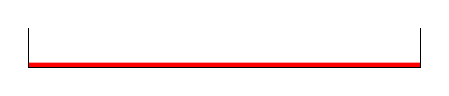
\begin{tikzpicture}\fill[red] (0.0,-6.25e-07) -- (0.0,0.0) -- (0.0,0.0625) -- (4.98046875,0.0625) -- (4.98046875,-6.25e-07) -- cycle;\draw (0,0.5) -- (0,0) -- (4.98046875,0) -- (4.98046875,0.5); \end{tikzpicture}                                                                                                                                                                                                                                                                                                                                                                                                                                                                                                                                                                                                                                                                                                                                                                                                                                                                                                                                                                                                                                                                                                                                     &3             &63              &4200              \\
Draper et al. (2004) \cite{draper2004lookaheadadder} &in    &Carry Lookahead         &$10n - 6\lg n - 13$              &$4\lg n + 7$                   &$2n - \lg n - 1$           &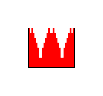
\begin{tikzpicture}\fill[red] (0.0,-6.25e-07) -- (0.0,0.0) -- (0.0,0.5) -- (0.01953125,0.5) -- (0.01953125,0.4375) -- (0.0390625,0.4375) -- (0.0390625,0.5) -- (0.05859375,0.5) -- (0.05859375,0.4375) -- (0.078125,0.4375) -- (0.078125,0.375) -- (0.09765625,0.375) -- (0.09765625,0.3125) -- (0.1171875,0.3125) -- (0.1171875,0.25) -- (0.13671875,0.25) -- (0.13671875,0.125) -- (0.17578125,0.125) -- (0.17578125,0.25) -- (0.1953125,0.25) -- (0.1953125,0.3125) -- (0.21484375,0.3125) -- (0.21484375,0.375) -- (0.234375,0.375) -- (0.234375,0.4375) -- (0.25390625,0.4375) -- (0.25390625,0.5) -- (0.2734375,0.5) -- (0.2734375,0.4375) -- (0.3125,0.4375) -- (0.3125,0.5) -- (0.33203125,0.5) -- (0.33203125,0.4375) -- (0.3515625,0.4375) -- (0.3515625,0.375) -- (0.37109375,0.375) -- (0.37109375,0.3125) -- (0.390625,0.3125) -- (0.390625,0.25) -- (0.41015625,0.25) -- (0.41015625,0.125) -- (0.44921875,0.125) -- (0.44921875,0.25) -- (0.46875,0.25) -- (0.46875,0.3125) -- (0.48828125,0.3125) -- (0.48828125,0.375) -- (0.5078125,0.375) -- (0.5078125,0.4375) -- (0.52734375,0.4375) -- (0.52734375,0.5) -- (0.546875,0.5) -- (0.546875,0.4375) -- (0.56640625,0.4375) -- (0.56640625,0.5) -- (0.5859375,0.5) -- (0.5859375,-6.25e-07) -- cycle;\draw (0,0.5) -- (0,0) -- (0.5859375,0) -- (0.5859375,0.5); \end{tikzpicture}       &17            &180             &1800              \\
Gidney (2017) \cite{gidney2018halving}               &in    &Ripple Carry            &$n - 1$                          &$2n - 1$                       &$n$                        &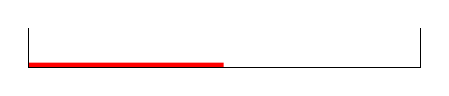
\begin{tikzpicture}\fill[red] (0.0,-6.25e-07) -- (0.0,0.0) -- (0.0,0.0625) -- (2.48046875,0.0625) -- (2.48046875,0.0) -- (4.98046875,0.0) -- (4.98046875,-6.25e-07) -- cycle;\draw (0,0.5) -- (0,0) -- (4.98046875,0) -- (4.98046875,0.5); \end{tikzpicture}                                                                                                                                                                                                                                                                                                                                                                                                                                                                                                                                                                                                                                                                                                                                                                                                                                                                                                                                                                                                                                                                                             &1             &76              &6600              \\
Mogensen (2019) \cite{mogensen2019lookahead}         &in    &Carry Lookahead         &$6n - 4$                         &$6\lg n + 2$                   &$n - \lg n - 1$            &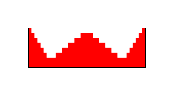
\begin{tikzpicture}\fill[red] (0.0,-6.25e-07) -- (0.0,0.0) -- (0.0,0.5) -- (0.0390625,0.5) -- (0.0390625,0.4375) -- (0.078125,0.4375) -- (0.078125,0.375) -- (0.1171875,0.375) -- (0.1171875,0.3125) -- (0.15625,0.3125) -- (0.15625,0.25) -- (0.1953125,0.25) -- (0.1953125,0.1875) -- (0.234375,0.1875) -- (0.234375,0.125) -- (0.3515625,0.125) -- (0.3515625,0.1875) -- (0.4296875,0.1875) -- (0.4296875,0.25) -- (0.5078125,0.25) -- (0.5078125,0.3125) -- (0.5859375,0.3125) -- (0.5859375,0.375) -- (0.6640625,0.375) -- (0.6640625,0.4375) -- (0.8203125,0.4375) -- (0.8203125,0.375) -- (0.8984375,0.375) -- (0.8984375,0.3125) -- (0.9765625,0.3125) -- (0.9765625,0.25) -- (1.0546875,0.25) -- (1.0546875,0.1875) -- (1.1328125,0.1875) -- (1.1328125,0.125) -- (1.25,0.125) -- (1.25,0.1875) -- (1.2890625,0.1875) -- (1.2890625,0.25) -- (1.328125,0.25) -- (1.328125,0.3125) -- (1.3671875,0.3125) -- (1.3671875,0.375) -- (1.40625,0.375) -- (1.40625,0.4375) -- (1.4453125,0.4375) -- (1.4453125,0.5) -- (1.484375,0.5) -- (1.484375,-6.25e-07) -- cycle;\draw (0,0.5) -- (0,0) -- (1.484375,0) -- (1.484375,0.5); \end{tikzpicture}                                                                                                                                                                                                     &14            &140             &1500              \\
Thapliyal et al (2020) \cite{thapliyal2020lookahead} &in    &Carry Lookahead         &$7n$*                            &$4\lg n + O(1)$*               &$2n$*                      &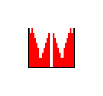
\begin{tikzpicture}\fill[red] (0.0,-6.25e-07) -- (0.0,0.0) -- (0.0,0.5) -- (0.01953125,0.5) -- (0.01953125,0.4375) -- (0.0390625,0.4375) -- (0.0390625,0.5) -- (0.05859375,0.5) -- (0.05859375,0.4375) -- (0.078125,0.4375) -- (0.078125,0.375) -- (0.09765625,0.375) -- (0.09765625,0.3125) -- (0.1171875,0.3125) -- (0.1171875,0.25) -- (0.13671875,0.25) -- (0.13671875,0.125) -- (0.17578125,0.125) -- (0.17578125,0.1875) -- (0.1953125,0.1875) -- (0.1953125,0.25) -- (0.21484375,0.25) -- (0.21484375,0.3125) -- (0.234375,0.3125) -- (0.234375,0.375) -- (0.25390625,0.375) -- (0.25390625,0.4375) -- (0.2734375,0.4375) -- (0.2734375,0.0) -- (0.3125,0.0) -- (0.3125,0.4375) -- (0.33203125,0.4375) -- (0.33203125,0.375) -- (0.3515625,0.375) -- (0.3515625,0.3125) -- (0.37109375,0.3125) -- (0.37109375,0.25) -- (0.390625,0.25) -- (0.390625,0.1875) -- (0.41015625,0.1875) -- (0.41015625,0.125) -- (0.44921875,0.125) -- (0.44921875,0.25) -- (0.46875,0.25) -- (0.46875,0.3125) -- (0.48828125,0.3125) -- (0.48828125,0.375) -- (0.5078125,0.375) -- (0.5078125,0.4375) -- (0.52734375,0.4375) -- (0.52734375,0.5) -- (0.546875,0.5) -- (0.546875,0.4375) -- (0.56640625,0.4375) -- (0.56640625,0.5) -- (0.5859375,0.5) -- (0.5859375,-6.25e-07) -- cycle;\draw (0,0.5) -- (0,0) -- (0.5859375,0) -- (0.5859375,0.5); \end{tikzpicture} &13            &130             &1300              \\
(this paper) (2020)                                  &in    &Blocksize=$\sqrt{n}$    &$5n + 6\sqrt{n} + O(1)$          &$6\sqrt{n} + 4\lg n + O(1)$    &$2n + 3\sqrt{n} + O(1)$    &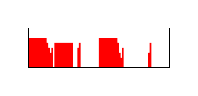
\begin{tikzpicture}\fill[red] (0.0,-6.25e-07) -- (0.0,0.0) -- (0.0,0.375) -- (0.234375,0.375) -- (0.234375,0.3125) -- (0.25390625,0.3125) -- (0.25390625,0.25) -- (0.2734375,0.25) -- (0.2734375,0.1875) -- (0.29296875,0.1875) -- (0.29296875,0.25) -- (0.3125,0.25) -- (0.3125,0.0) -- (0.33203125,0.0) -- (0.33203125,0.3125) -- (0.56640625,0.3125) -- (0.56640625,0.0) -- (0.625,0.0) -- (0.625,0.25) -- (0.64453125,0.25) -- (0.64453125,0.3125) -- (0.6640625,0.3125) -- (0.6640625,0.0) -- (0.8984375,0.0) -- (0.8984375,0.375) -- (1.1328125,0.375) -- (1.1328125,0.3125) -- (1.15234375,0.3125) -- (1.15234375,0.1875) -- (1.171875,0.1875) -- (1.171875,0.125) -- (1.19140625,0.125) -- (1.19140625,0.25) -- (1.2109375,0.25) -- (1.2109375,0.0) -- (1.5234375,0.0) -- (1.5234375,0.1875) -- (1.54296875,0.1875) -- (1.54296875,0.3125) -- (1.5625,0.3125) -- (1.5625,0.0) -- (1.796875,0.0) -- (1.796875,-6.25e-07) -- cycle;\draw (0,0.5) -- (0,0) -- (1.796875,0) -- (1.796875,0.5); \end{tikzpicture}                                                                                                                                                                                                                                                                                                                                     &10            &97              &950               \\
(this paper) (2020)                                  &in    &Blocksize=b             &$5n - 4b + 10\frac{n}{b} + O(1)$ &$6b + 8\lg \frac{n}{b} + O(1)$ &$2n + 3\frac{n}{b} + O(1)$ &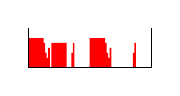
\begin{tikzpicture}\fill[red] (0.0,-6.25e-07) -- (0.0,0.0) -- (0.0,0.375) -- (0.1953125,0.375) -- (0.1953125,0.3125) -- (0.21484375,0.3125) -- (0.21484375,0.1875) -- (0.234375,0.1875) -- (0.234375,0.125) -- (0.25390625,0.125) -- (0.25390625,0.25) -- (0.2734375,0.25) -- (0.2734375,0.0) -- (0.29296875,0.0) -- (0.29296875,0.3125) -- (0.48828125,0.3125) -- (0.48828125,0.0) -- (0.546875,0.0) -- (0.546875,0.1875) -- (0.56640625,0.1875) -- (0.56640625,0.3125) -- (0.5859375,0.3125) -- (0.5859375,0.0) -- (0.78125,0.0) -- (0.78125,0.375) -- (0.9765625,0.375) -- (0.9765625,0.3125) -- (0.99609375,0.3125) -- (0.99609375,0.1875) -- (1.015625,0.1875) -- (1.015625,0.125) -- (1.03515625,0.125) -- (1.03515625,0.25) -- (1.0546875,0.25) -- (1.0546875,0.0) -- (1.328125,0.0) -- (1.328125,0.1875) -- (1.34765625,0.1875) -- (1.34765625,0.3125) -- (1.3671875,0.3125) -- (1.3671875,0.0) -- (1.5625,0.0) -- (1.5625,-6.25e-07) -- cycle;\draw (0,0.5) -- (0,0) -- (1.5625,0) -- (1.5625,0.5); \end{tikzpicture}                                                                                                                                                                                                                                                                                                                           &9             &96              &950               \\

\hline
Gossett (1998) \cite{gossett1998carrysave}           &out   &Carry Save (avg over n) &$4n$                             &$2$                            &$n^2 - 2n$                 &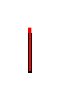
\begin{tikzpicture}\fill[red] (0.0,-6.25e-07) -- (0.0,0.0) -- (0.0,0.5625) -- (0.0390625,0.5625) -- (0.0390625,-6.25e-07) -- cycle;\draw (0,0.5) -- (0,0) -- (0.0390625,0) -- (0.0390625,0.5); \end{tikzpicture}                                                                                                                                                                                                                                                                                                                                                                                                                                                                                                                                                                                                                                                                                                                                                                                                                                                                                                                                                                                                                                                                                                                                         &71            &6600            &660000            \\
Draper et al. (2004) \cite{draper2004lookaheadadder} &out   &Carry Lookahead         &$5n - 3\lg n - 4$                &$2\lg n + 3$                   &$n - \lg n$                &
\begin{tikzpicture}\fill[red] (0.0,-6.25e-07) -- (0.0,0.0) -- (0.0,0.5) -- (0.01953125,0.5) -- (0.01953125,0.4375) -- (0.0390625,0.4375) -- (0.0390625,0.5) -- (0.05859375,0.5) -- (0.05859375,0.4375) -- (0.078125,0.4375) -- (0.078125,0.375) -- (0.09765625,0.375) -- (0.09765625,0.3125) -- (0.1171875,0.3125) -- (0.1171875,0.25) -- (0.13671875,0.25) -- (0.13671875,0.125) -- (0.17578125,0.125) -- (0.17578125,0.25) -- (0.1953125,0.25) -- (0.1953125,0.3125) -- (0.21484375,0.3125) -- (0.21484375,0.375) -- (0.234375,0.375) -- (0.234375,0.4375) -- (0.25390625,0.4375) -- (0.25390625,0.5) -- (0.2734375,0.5) -- (0.2734375,0.4375) -- (0.29296875,0.4375) -- (0.29296875,-6.25e-07) -- cycle;\draw (0,0.5) -- (0,0) -- (0.29296875,0) -- (0.29296875,0.5); \end{tikzpicture}                                                                                                                                                                                                                                                                                                                                                                                                                                                                                                                                                               &8             &91              &920               \\
Gidney (2017) \cite{gidney2018halving}               &out   &Ripple Carry            &$n - 1$                          &$n - 1$                        &$1$                        &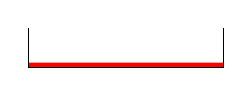
\begin{tikzpicture}\fill[red] (0.0,-6.25e-07) -- (0.0,0.0) -- (0.0,0.0625) -- (2.48046875,0.0625) -- (2.48046875,-6.25e-07) -- cycle;\draw (0,0.5) -- (0,0) -- (2.48046875,0) -- (2.48046875,0.5); \end{tikzpicture}                                                                                                                                                                                                                                                                                                                                                                                                                                                                                                                                                                                                                                                                                                                                                                                                                                                                                                                                                                                                                                                                                                                                     &1             &41              &3100              \\
Mogensen (2019) \cite{mogensen2019lookahead}         &out   &Carry Lookahead         &$12n - 8$                        &$12\lg n + 4$                  &$n - \lg n - 1$            &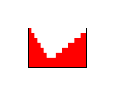
\begin{tikzpicture}\fill[red] (0.0,-6.25e-07) -- (0.0,0.0) -- (0.0,0.5) -- (0.0390625,0.5) -- (0.0390625,0.4375) -- (0.078125,0.4375) -- (0.078125,0.375) -- (0.1171875,0.375) -- (0.1171875,0.3125) -- (0.15625,0.3125) -- (0.15625,0.25) -- (0.1953125,0.25) -- (0.1953125,0.1875) -- (0.234375,0.1875) -- (0.234375,0.125) -- (0.3515625,0.125) -- (0.3515625,0.1875) -- (0.4296875,0.1875) -- (0.4296875,0.25) -- (0.5078125,0.25) -- (0.5078125,0.3125) -- (0.5859375,0.3125) -- (0.5859375,0.375) -- (0.6640625,0.375) -- (0.6640625,0.4375) -- (0.7421875,0.4375) -- (0.7421875,-6.25e-07) -- cycle;\draw (0,0.5) -- (0,0) -- (0.7421875,0) -- (0.7421875,0.5); \end{tikzpicture}                                                                                                                                                                                                                                                                                                                                                                                                                                                                                                                                                                                                                                                                 &19            &190             &1900              \\
Thapliyal et al (2020) \cite{thapliyal2020lookahead} &out   &Carry Lookahead         &$4n$                             &$2\lg n + O(1)$                &$2n$*                      &
\begin{tikzpicture}\fill[red] (0.0,-6.25e-07) -- (0.0,0.0) -- (0.0,0.5) -- (0.01953125,0.5) -- (0.01953125,0.4375) -- (0.0390625,0.4375) -- (0.0390625,0.5) -- (0.05859375,0.5) -- (0.05859375,0.4375) -- (0.078125,0.4375) -- (0.078125,0.375) -- (0.09765625,0.375) -- (0.09765625,0.3125) -- (0.1171875,0.3125) -- (0.1171875,0.25) -- (0.13671875,0.25) -- (0.13671875,0.125) -- (0.17578125,0.125) -- (0.17578125,0.1875) -- (0.1953125,0.1875) -- (0.1953125,0.25) -- (0.21484375,0.25) -- (0.21484375,0.3125) -- (0.234375,0.3125) -- (0.234375,0.375) -- (0.25390625,0.375) -- (0.25390625,0.4375) -- (0.2734375,0.4375) -- (0.2734375,0.0) -- (0.29296875,0.0) -- (0.29296875,-6.25e-07) -- cycle;\draw (0,0.5) -- (0,0) -- (0.29296875,0) -- (0.29296875,0.5); \end{tikzpicture}                                                                                                                                                                                                                                                                                                                                                                                                                                                                                                                                                               &7             &80              &800               \\
(this paper) (2020)                                  &out   &Blocksize=$\sqrt{n}$    &$3n + 3\sqrt{n} + O(1)$          &$3\sqrt{n} + 2\lg n + O(1)$    &$2n + 3\sqrt{n} + O(1)$    &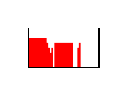
\begin{tikzpicture}\fill[red] (0.0,-6.25e-07) -- (0.0,0.0) -- (0.0,0.375) -- (0.234375,0.375) -- (0.234375,0.3125) -- (0.25390625,0.3125) -- (0.25390625,0.25) -- (0.2734375,0.25) -- (0.2734375,0.1875) -- (0.29296875,0.1875) -- (0.29296875,0.25) -- (0.3125,0.25) -- (0.3125,0.0) -- (0.33203125,0.0) -- (0.33203125,0.3125) -- (0.56640625,0.3125) -- (0.56640625,0.0) -- (0.625,0.0) -- (0.625,0.25) -- (0.64453125,0.25) -- (0.64453125,0.3125) -- (0.6640625,0.3125) -- (0.6640625,0.0) -- (0.8984375,0.0) -- (0.8984375,-6.25e-07) -- cycle;\draw (0,0.5) -- (0,0) -- (0.8984375,0) -- (0.8984375,0.5); \end{tikzpicture}                                                                                                                                                                                                                                                                                                                                                                                                                                                                                                                                                                                                                                                                                                                       &6             &63              &610               \\
(this paper) (2020)                                  &out   &Blocksize=b             &$3n - 2b + 5\frac{n}{b} + O(1)$  &$3b + 4\lg \frac{n}{b} + O(1)$ &$2n + 3\frac{n}{b} + O(1)$ &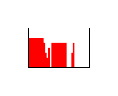
\begin{tikzpicture}\fill[red] (0.0,-6.25e-07) -- (0.0,0.0) -- (0.0,0.375) -- (0.1953125,0.375) -- (0.1953125,0.3125) -- (0.21484375,0.3125) -- (0.21484375,0.1875) -- (0.234375,0.1875) -- (0.234375,0.125) -- (0.25390625,0.125) -- (0.25390625,0.25) -- (0.2734375,0.25) -- (0.2734375,0.0) -- (0.29296875,0.0) -- (0.29296875,0.3125) -- (0.48828125,0.3125) -- (0.48828125,0.0) -- (0.546875,0.0) -- (0.546875,0.1875) -- (0.56640625,0.1875) -- (0.56640625,0.3125) -- (0.5859375,0.3125) -- (0.5859375,0.0) -- (0.78125,0.0) -- (0.78125,-6.25e-07) -- cycle;\draw (0,0.5) -- (0,0) -- (0.78125,0) -- (0.78125,0.5); \end{tikzpicture}                                                                                                                                                                                                                                                                                                                                                                                                                                                                                                                                                                                                                                                                                                             &6             &62              &610               \\
\end{tabular}
